\pdfoutput=1

\documentclass[11pt]{article}

\usepackage[]{acl}

\usepackage{times}
\usepackage{latexsym}

\usepackage[T1]{fontenc}

\usepackage[utf8]{inputenc}

\usepackage{microtype}


\usepackage[pdftex]{graphicx}
\usepackage{tabularx}
\usepackage{amsmath}
\usepackage{bm}
\usepackage{array}
\usepackage{enumitem}
\usepackage{wrapfig}
\usepackage{caption}
\usepackage{subcaption}
\usepackage{amsmath,amsfonts,bm}

\usepackage{booktabs}
\usepackage{multirow}
\usepackage[normalem]{ulem}
\useunder{\uline}{\ul}{}

\usepackage{algorithm}
\usepackage{algorithmic}
\renewcommand{\algorithmicrequire}{\textbf{Input:}}
\renewcommand{\algorithmicensure}{\textbf{Output:}}

\newcommand{\E}{\mathbb{E}}
\newcommand{\KLD}{\text{KL}}
\newcommand{\ENT}{\text{H}}
\newcommand{\BENT}{\mathbb{H}}
\newcommand{\BDist}{\mathbb{D}}
\newcommand{\MLE}{\text{MLE}}
\newcommand{\x}{\bm{x}}
\newcommand{\y}{\bm{y}}
\newcommand{\z}{\bm{z}}
\newcommand{\s}{\bm{s}}
\newcommand{\ba}{\bm{a}}
\newcommand{\bt}{\bm{t}}
\newcommand{\bc}{\bm{c}}
\newcommand{\yspace}{\mathcal{Y}}
\newcommand{\zspace}{\mathcal{Z}}
\newcommand{\tspace}{\mathcal{T}}
\newcommand{\btheta}{\bm{\theta}}
\newcommand{\bphi}{\bm{\phi}}
\newcommand{\bxi}{\bm{\xi}}
\newcommand{\bw}{\bm{\w}}
\newcommand{\dataset}{\mathcal{D}}
\newcommand{\loss}{\mathcal{L}}
\newcommand{\indicator}{\mathbb{I}}
\newcommand{\pdata}{p_{d}}
\newcommand{\pemp}{\tilde{p}_d}
\newcommand{\lm}{\text{LM}}









\title{
Efficient (Soft) $Q$-Learning \\ for Text Generation
with Limited Good Data
}


\author{
Han Guo$^1$,~~
Bowen Tan$^1$,~~
Zhengzhong Liu$^{1,2}$,~~
Eric P. Xing$^{1,2,4}$,~~
Zhiting Hu$^{3}$\\
$^1$Carnegie Mellon University,~~ $^2$Petuum Inc.,~~ $^3$UC San Diego,\\
$^4$Mohamed bin Zayed University of Artificial Intelligence\\
{\small 
{\tt \{hanguo, btan2, epxing\}@cs.cmu.edu, hectorzliu@gmail.com, zhh019@ucsd.edu}
}
}

\begin{document}
\maketitle
\begin{abstract}
Maximum likelihood estimation (MLE) is the predominant algorithm for training text generation models. This paradigm relies on direct supervision examples, which is not applicable to many emerging applications, such as generating adversarial attacks or generating prompts to control language models. Reinforcement learning (RL) on the other hand offers a more flexible solution by allowing users to plug in arbitrary task metrics as reward. Yet previous RL algorithms for text generation, such as policy gradient (\emph{on-policy} RL) and $Q$-learning (\emph{off-policy} RL), are often notoriously inefficient or unstable to train due to the large sequence space and the sparse reward received only at the end of sequences. In this paper, we introduce a new RL formulation for text generation from the soft $Q$-learning (SQL) perspective. It enables us to draw from the latest RL advances, such as path consistency learning, to combine the best of on-/off-policy updates, and learn effectively from sparse reward. We apply the approach to a wide range of novel text generation tasks, including learning from noisy/negative examples, adversarial attacks, and prompt generation. Experiments show our approach consistently outperforms both task-specialized algorithms and the previous RL methods.%
\footnote{Code at \url{https://github.com/HanGuo97/soft-Q-learning-for-text-generation}.}
\end{abstract}


\section{Introduction}

In the most simple case, time series forecasting deals with a scalar
time-varying signal and aims to predict or forecast its values in the near future; for example, countless applications in finance, healthcare, production automatization, etc. \cite{cao2018brits,sagheer2019time,sezer2020financial} can benefit from an accurate forecasting solution.
Often not just a single scalar signal is of interest, but multiple at once,
and further time-varying signals are available and even \textsl{known for the future}.
For example, suppose one aims to forecast the energy consumption of a house, it likely depends on the social time that one seeks to forecast for (such as the next hour or day), and also on features of these time points (such as weekday, daylight, etc.), which are known already for the future. This is also the case in model predictive control \cite{camacho2013model}, where one is interested
to forecast the expected value realized by some planned action, then this action is also known at the time of forecast.
More generally,
time series forecasting, nowadays deals with quadruples $(x,y,x',y')$
of known past predictors $x$, known past targets $y$, known future predictors $x'$
and sought future targets $y'$. 

\begin{figure}[ht]
\centering

\includegraphics[width=0.4\columnwidth]{figs/ts_ps.png}
\caption{General time series setting illustrating the quadruples $(x,y,x',y')$ denoting the \textsl{past predictors}, \textsl{past targets}, \textsl{future predictors} and \textsl{future targets} respectively. Given the history information $(x, y)$ until time $t = T$ and the future predictors $(x')$ for the next $\tau$ time steps, time series forecasting predicts the target $y'$ from $t = T+1, \dots, \tau$ time steps. In the figure, $O$ and $M$ represents the respective channels of the targets and the predictors.}
\label{fig:ts_ps}
\end{figure}

Time series problems can often be addressed by methods developed initially
for images, treating them as 1-dimensional images. Especially for
time-series classification many typical time series encoder architectures
have been adapted from models for images \cite{wang2017time,ZOU201939}. 
Time series forecasting then is closely related to image outpainting \cite{wang2019srn},
the task to predict how an image likely extends to the left, right, top or bottom,
as well as to the more well-known task of image segmentation,
where for each input pixel, an output pixel has to be predicted, whose channels
encode pixel-wise classes such as vehicle, road, pedestrian say for road scenes.
Time series forecasting combines aspects from both problem settings:
information about targets from shifted positions (e.g., the past targets $y$ as
 in image outpainting) and
information about other channels from the same positions (e.g., the future predictors $x'$
 as in image segmentation).
One of the most successful, principled architectures for the image segmentation
task are U-Nets introduced in \cite{ronneberger2015u}, an architecture that successively downsamples/coarsens
its inputs and then upsamples/refines the latent representation with
deconvolutions also using the latent representations of the same detail level,
tightly coupling down- and upsampling procedures and thus yielding latent
features on the same resolution as the inputs. 


Following the great success in Natural Language Processing (NLP) applications, attention-based, esp. transformer-based
architectures \cite{vaswani2017attention} that model pairwise interactions
between sequence elements have been recently adapted for
time series forecasting. One of the significant
challenges, is that the length of the time series, are often one or two magnitudes of order larger than the (sentence-level) NLP problems. 

Plenty of approaches aim to mitigate the quadratic complexity $O(T^2)$ in
the sequence/time series length $T$ to at most $O(T\log T)$.
For example, the Informer architecture
\cite{zhou2020informer}, adapts the transformer with a sparse attention
mechanism and a successive downsampling/coarsening of the past time series. As in the original transformer, only the coarsest representation is fed
into the decoder. Possibly to remedy the loss in resolution by this procedure,
the Informer feeds its input a second time into the decoder network, this time
without any coarsening. 

While forecasting problems share many commonalities with image segmentation
problems, transformer-based architectures like the Informer do not
involve coupled down- and upscaling procedures to yield predictions
on the same resolution as the inputs. 
Thus, we propose a novel Y-shaped architecture that
\begin{enumerate}
\item Couples downscaling/upscaling to leverage both, coarse and fine-grained
       features for time series forecasting,
\item Combines the coupled scaling mechanism with sparse attention modules to capture long-range effects on all scale levels, and
\item Stabilizes encoder and decoder stacks by reconstructing the recent past.
\end{enumerate}






\section{Background and Challenges}
\label{subsec:preliminaries}

We aim to learn a generation model
$p_{\theta} (\y) = \prod_{t=0}^T p_{\theta}(y_t | \y_{<t})$, where
$y_t$ is a token from a vocabulary $\mathcal{V}$. The distribution at each step $t$ is obtained by applying softmax on the logits $f_\theta(y | \y_{<t})$:
\begin{equation}
\small
\begin{split}
    p_\theta(y_t | \y_{<t}) = \frac{\exp f_\theta(y_t | \y_{<t}) }{ \sum_{y'\in\mathcal{V}} \exp f_\theta(y' | \y_{<t} ) }.
\end{split}
\label{eq:softmax-logit}
\end{equation}
Despite its popularity, MLE-based training only applies when clean supervised data $\bm{y}^*$ is available, and cannot be used to optimize arbitrary task metrics (e.g., BLEU, entailment score) which are typically the goal in many text generation tasks. 
\label{sec:background:rl}
Previous research has formulated text generation as an RL problem by considering the following finite-time Markov Decision Process (MDP). 
At each time step $t$, let the ``state'' be $\bm{s}_t = \bm{y}_{< t}$, namely the partial sequence generated so far. The model (``agent'') takes as input the current state $\bm{s}_t$ and outputs a token (``action'') $a_t \in \mathcal{V}$ according to a policy $\pi(a_t | \bm{s}_t)$. 
The agent then receives a reward $r_t = r(\bm{s}_t, a_t)$ and deterministically transitions to next state $\bm{s}_{t+1}$ (i.e., the concatenation of the tokens in $\s_t$ and the new token $a_t$). 

Following the notation convention in RL, let $\tau$ be the trajectory (i.e., text sample) generated by the policy. The agent's objective is to maximize the accumulative reward,
$J(\pi) = \mathbb{E}_{\tau \sim \pi}\left[ \sum^T_{t=0} \gamma^t r_t \right]$,
where $\gamma$ is the discount factor.
A central concept in RL is the $Q$-function of policy $\pi$, $Q^\pi(\s_t, a_t)=\E_{\pi}\left[ \sum_{t'=t}^T \gamma^{t'} r_{t'} \mid \s_t, a_t \right]$, the expected future reward of taking action $a_t$ (i.e., generating token $a_t$) in state $\s_t$ and continuing with the policy $\pi$. 

\noindent\textbf{Challenges. } Text generation poses significant challenges to RL, particularly because (1) the reward signal is usually sparse, i.e., $r_t = 0,\ \forall t<T$ and the agent receives a non-zero reward $r_{T}$ only after it generates the full sequence, (2) the action space (i.e., the vocabulary $\mathcal{V}$) is extremely large.
The challenges have led to difficulties of the two major families of RL approaches applied to text generation problems, as detailed below.

\noindent\textbf{Policy-based RL}
techniques directly parameterize the policy $\pi_{\theta}$ with parameters $\btheta$. Thus the policy $\pi_{\theta}(a_t | \s_t)$ exactly corresponds to the above generation model $p_{\theta}(y_t | \y_{<t})$. 
\emph{Policy gradient (PG)} is one of the most widely used algorithms for text generation \citep{ranzato2015sequence}.
It optimizes the cumulative reward with the policy gradient using the estimated $Q^{\pi_\theta}$ value based on sample $\tau$. PG is an \textit{on-policy} algorithm, meaning that the sample $\tau$ needs to come from the the current policy $\pi_\theta$ itself.
In practice, however, optimizing this objective alone from scratch is unlikely going to work because most samples $\tau\sim\pi_\theta$ are just gibberish with zero reward, failing to provide meaningful training signals for updating the policy. 
Previous literature either initializes the policy $\pi_{{\theta}}$ with MLE training, and/or use a combination of MLE and PG updates, which often leads to marginal gains in practice~\citep{wu2018study,Choshen2020On}. 



\noindent\textbf{Value-based RL}
techniques, such as \emph{$Q$-learning}, implicitly learn the policy $\pi$ by approximating the value $Q^{\pi}(\bm{s}, a)$ directly.
Deep $Q$-learning~\citep{mnih2013playing} parameterizes the $Q$-function as $Q_\theta(\x,a)$, and train the parameters by minimizing the following regression objective $\loss(\btheta)$ based on the Bellman temporal consistency:
\begin{equation}
\small
    {\E}_{\pi'}\left[ \frac{1}{2} \left( r_t {+} \gamma \max_{a_{t+1}} Q_{\bar{\theta}}(\s_{t+1}, a_{t+1}) {-} Q_{\theta}(\s_t, a_t) \right)^2 \right]%
\label{eq:q-regression}
\end{equation}
where $\bar{\btheta}$ is the parameters of the \emph{target} $Q$-network, which is a slow copy of $\btheta$ and considered as constant for gradient computation of $\btheta$. 
Here $\pi'$ is an \emph{behavior policy} which can be an arbitrary distribution over text, such as the data distribution or replay buffer \citep{mnih2013playing}. 
This makes $Q$-learning an \textit{off-policy} algorithm because of its ability to use samples coming from other policies. After learning $Q_\theta$, one can induce a policy $\pi$ from it that takes $\arg\max_{a} Q_\theta(\s, a)$ at each state $\s$.
\citet{jaques2017sequence} instead sample tokens from the softmax function applied to $Q_\theta$.

However, the training can be unstable and inefficient due to several challenges: 
{\bf (1)} The bootstrapping nature of the above regression problem can make the training unstable. That is, the regression target $r_t + \gamma \max_{a_{t+1}} Q_{\bar{\theta}}(\s_{t+1}, a_{t+1})$ itself is derived from the $Q$-function to be learned \citep{kumar2019stabilizing}. The problem is exacerbated in the presence of sparse reward in text generation, where the real observed signal $r_t$ is zero for all intermediate $t<T$; 
{\bf (2)} The large action space (e.g., $10^4$) in text generation results in slow updates. In particular, notice that Eq.\eqref{eq:q-regression} applies the gradient update to the $Q_{{\theta}}$-value of the \emph{only one} particular token $a_t$ (out of, say, the $10^4$ candidate tokens in the vocabulary), making the training inefficient;
{\bf (3)} Besides, pure off-policy updates could be highly sensitive to the quality of training data, and miss the opportunity of on-policy exploration that maximizes the reward of interest in a more direct way.



\begin{figure*}
    \centering
    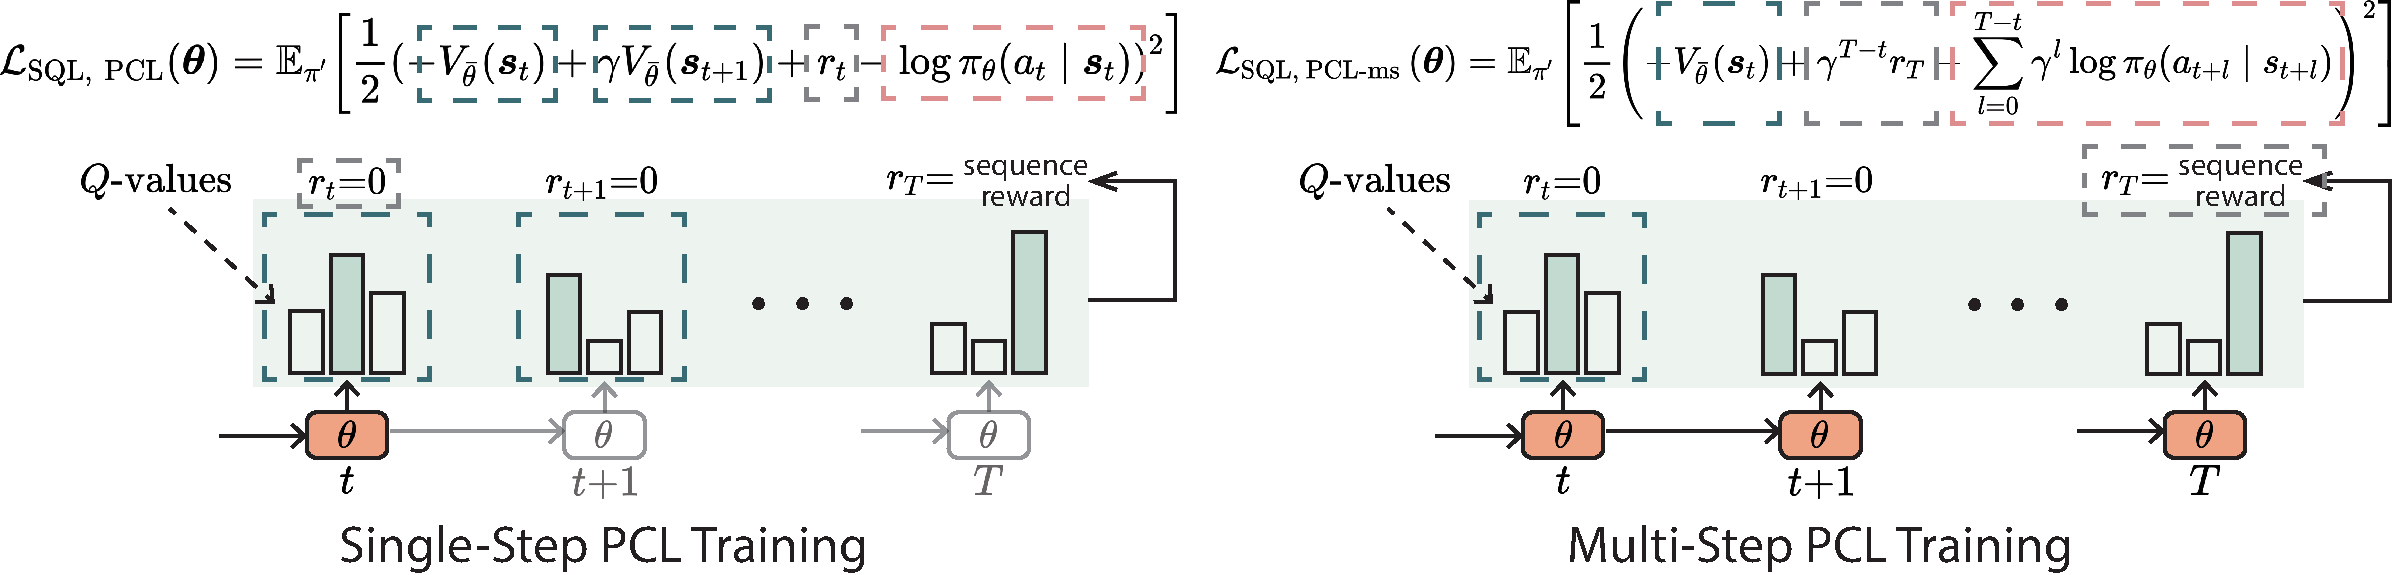
\includegraphics[width=0.99\linewidth]{figures/soft-q-learning.pdf}
    \vspace{-4pt}
    \caption{
    Soft $Q$-Learning with path consistency learning (PCL) objectives.
    {\bf Left:} Single-step objective (Eq.\ref{eq:pcl-loss}), where for each $(\s_t, a_t)$, the computation involves step $t$ and $t+1$. Dashed boxes in \textcolor[HTML]{3A6B73}{\textbf{dark green}} and \textcolor[HTML]{808285}{\textbf{gray}} indicate the regression target, where the intermediate reward $r_t$ is often 0 due to sparsity. The gradient is applied to parameters $\btheta$ at step $t$ (indicated by {\textcolor{orange}{\textbf{orange}}} color). {\bf Right:} Multi-step objective (Eq.\ref{eq:multi-loss}) which aggregates from step $t$ all the way to $T$. In this way, the final-step non-zero reward $r_T$ is used as the regression target.
    }
    \vspace{-4pt}
    \label{fig:soft-q-learning-pcl}
\end{figure*}



\section{The Soft $Q$-Learning Framework}


We introduce the soft $Q$-learning (SQL) formulation of text generation. It is seamlessly compatible with the common architecture of text generation model (Eq.\ref{eq:softmax-logit}), permits easy implementation (\S\ref{sec:sql-formulation}),
and enables efficient and stable RL training in practice (\S\ref{subsec:method:pcl}).
Figure~\ref{fig:soft-q-learning-pcl} and Algorithm~\ref{alg:sql} summarizes the resulting SQL framework.




\subsection{SQL Formulation for Text Generation}\label{sec:sql-formulation}

Soft $Q$-learning \citep{haarnoja2017reinforcement,schulman2017equivalence,nachum2017bridging} is an maximum-entropy (MaxEnt) extension to the standard (hard) $Q$-learning~\citep{mnih2015human,sutton2018reinforcement}. Under this framework, the agent is encouraged to optimize the reward while staying as stochastic as possible, with the objective
$J_{\text{MaxEnt}}(\pi)=\mathbb{E}_{\tau \sim \pi}\left[\sum_{t=0}^T \gamma^t r_t + \alpha \mathcal{H}\left(\pi\left(\cdot \mid \bm{s}_{t}\right)\right)\right]$,
which augments the vanilla $J(\pi)$
with the additional Shannon entropy term $\mathcal{H}$ with coefficient $\alpha$.\footnote{WLOG, we can assume $\alpha{=}1$, as it can be folded into the reward function by scaling the latter with $1/\alpha$.}
This is appealing because it seamlessly connects the $Q$-values to the familiar output \textit{logits} of a text generation model, which enables straightforward implementation of the SQL formulation.

\noindent\textbf{$Q$-values as Generation Model Logits.}
We show the connection of the $Q$-values with the logits, i.e., outputs right before the $\operatorname{softmax}$ layer.
Concretely, with the SQL objective,
the following relationship between optimal policy $\pi^*$ and action-value $Q^*$ holds~\citep{haarnoja2017reinforcement,schulman2017equivalence}:
\begin{equation}
\small
    \pi^{*}(a | \bm{s})=\frac{\exp Q^{*}(\bm{s}, a)}{\sum_{a^{\prime}} \exp Q^{*}\left(\bm{s}, a^{\prime}\right)}.
    \label{eq:optimal-pi-and-q}
\end{equation}
This form is highly reminiscent of the $\operatorname{softmax}$ layer of the generation model in Eq.\eqref{eq:softmax-logit}. The connection suggests that we can naturally parameterize the $Q$-function in SQL as the generation model logit function, i.e., $Q_\theta(\s, a) \equiv f_\theta(a|\s)$. In other words, \emph{the model output $f_\theta(a|\s)$, originally interpretted as the ``logit'' of token $a$ given the preceding tokens $\s$, is now re-interpretted as the $Q$-value of action $a$ in state $\s$.} When achieving optimality, $f_{\theta^*}(a|\s)$, namely $Q^{*}(\bm{s}, a)$, represents the best possible future reward achievable by generating token $a$ in state $\bm{s}$. Similarly, the full generation model $p_\theta(a|\s)$ in Eq.\eqref{eq:softmax-logit} that applies $\operatorname{softmax}$ to $f_\theta$ now precisely corresponds to the policy $\pi_\theta$ induced from $Q_\theta(\s, a)$. That is,
\begin{equation}
\small
\begin{aligned}
    \pi_\theta(a | \bm{s})
    &= \frac{\exp Q_\theta(\bm{s}, a)}{\sum_{a^{\prime}} \exp Q_\theta\left(\bm{s}, a^{\prime}\right)} \\
    &\equiv \frac{\exp f_\theta(a | \bm{s})}{\sum_{a^{\prime}} \exp f_\theta\left(a^{\prime} | \bm{s} \right)} 
    = p_\theta(a | \s).
    \label{eq:pi-and-q-theta}
\end{aligned}
\end{equation}
We could further gain even more intuitive interpretation of the above generation policy $\pi^*$ from the lens of \emph{advantage} function  \citep{sutton2018reinforcement}. Specifically, in SQL, the optimal \emph{state-value} function is the log-normalizer of the optimal $Q$-values \citep{haarnoja2017reinforcement,schulman2017equivalence}.
This allows a more concise form of Eq.\eqref{eq:optimal-pi-and-q}:
\begin{equation}
\small
\begin{aligned}
    V^{*}\left(\bm{s}\right) &= \log \sum\nolimits_{a'} \exp Q^{*}\left(\bm{s}, a'\right) \\ %
    \pi^{*}(a | \bm{s}) &= \exp \big(Q^*(\bm{s}, a) - V^*(\bm{s})\big) = \exp A^*(\bm{s}, a),
    \label{eq:sql-state-value}
\end{aligned}
\end{equation}
where $A^*$ is the optimal advantage function. The equation says that, in the proposed text generation SQL formulation, the optimal policy generates token $a$ in state $\s$ according to the token's advantage.







\subsection{Efficient Training with Path Consistency}
\label{subsec:method:pcl}

Vanilla training based on the Bellman temporal consistency can suffer from the instability and inefficiency issues similar to the conventional $Q$-learning (\S\ref{sec:background:rl}), as we discuss more in the appendix (\S\ref{appendix-subsubsec:vanilla-training-with-temporal-consistency}). Fortunately, our SQL formulation allows us to import latest advances of RL techniques to overcome the difficulties.
Specifically, we adapt the \emph{unified path consistency learning (PCL)} that has excelled in game control~\citep{nachum2017bridging}.
The PCL-based training updates $Q$-values of \emph{all} tokens at once through a connection between the value function and the induced policy.
More specifically,~\citet{nachum2017bridging} showed that the optimal policy $\pi^*$ (Eq.\ref{eq:optimal-pi-and-q}) and the optimal state value function $V^*$ (Eq.\ref{eq:sql-state-value}) in SQL must satisfy the following consistency property for 
all states and actions:
\begin{equation}
\small
    V^*\left(\bm{s}_{t}\right)-\gamma V^*\left(\bm{s}_{t+1}\right) = r_t - \log \pi^*\left(a_{t} | \bm{s}_{t}\right), \forall \bm{s}_t,\  a_t.
    \label{eq:pcl}
\end{equation}
Accordingly, the PCL-based training attempts to encourage the satisfaction of the consistency with the following regression objective $\loss_{\text{SQL, PCL}} (\bm{\theta})$:
\begin{equation}
\small
\begin{aligned}
    {\mathbb{E}}_{\pi'}\left[\frac{1}{2}\bigg({-}V_{\bar{{\theta}}}\left(\bm{s}_{t}\right){+}\gamma V_{\bar{{\theta}}}\left(\bm{s}_{t+1}\right) {+} 
    r_t {-} \log \pi_{{\theta}}\left(a_{t} | \bm{s}_{t}\right)\bigg)^{2}\right],
    \label{eq:pcl-loss}
\end{aligned}
\end{equation}
where $\pi_\theta$ is the induced policy defined in Eq.\eqref{eq:pi-and-q-theta}; $V_{\bar{{\theta}}}$ is defined similarly as in Eq.\eqref{eq:sql-state-value} but depends on the target $Q_{\bar{\theta}}$ network (i.e., a slow copy of the $Q_\theta$ to be learned), and recall that $\pi'$ is an arbitrary behavior policy (e.g., data distribution). 
Please see Figure~\ref{fig:soft-q-learning-pcl} (left) for an illustration. 
Crucially, notice that the gradient update is applied to $\btheta$ through the $\log \pi_\theta$ term which explicitly involves the $Q_\theta$-values of \emph{all} tokens $a$ in the vocabulary. This shows an important difference from the above vanilla training in conventional $Q$-learning (\S\ref{sec:background:rl}) where $Q_\theta$ is updated only through the particular $a_t$ token. The PCL training thus offers more efficient updates for the $Q_\theta$ function.
In the appendix (\S\ref{comparison-with-mle-objective}), we also discuss the difference from the MLE objective. Intuitively, MLE trains the model to (blindly) increase the probability of the observed tokens, while PCL encourages the (log) probability of the tokens to match the approximate advantage values.



\paragraph{Multi-step PCL for Sparse Reward.} 
The above PCL objective Eq.\eqref{eq:pcl-loss} alone does not resolve the potential instability issue due to the bootstrapped $V_{\bar{{\theta}}}(\s_{t+1})$ value and the sparse reward (i.e., $r(\s_t, a_t)=0$ for $t<T$). 
Our SQL formulation allows us to additionally incorporate the \emph{multi-step} variant of the PCL training \citep{nachum2017bridging} to resolve the issue. Specifically, by applying a telescoping sum on the consistency equation (Eq.\ref{eq:pcl}) starting from $t$ up to $T$, we arrive at the multi-step temporal consistency:
\begin{equation}
\small
\begin{aligned}
    &V^{*}\left(\bm{s}_{t}\right){-}\gamma^{T-t} V^{*}\left(\bm{s}_{T+1}\right)
    {=} \sum_{l=t}^{T} \gamma^{l-t}\big(r_{l}{-}\log \pi^{*}\left(a_{l} | \bm{s}_{l}\right)\big),
\end{aligned}
\end{equation}
where the value of past-terminal state is zero, $V^*\left(\bm{s}_{T+1}\right) = 0$; and the rewards are only available at the end, $\sum_{l=t}^{T} \gamma^{l-t} r_{l} = \gamma^{T-t} r_{T}$. We can then come to the following multi-step objective function $\loss_{\textrm{SQL, PCL-ms}}(\btheta)$, 
\begin{equation}
\small
    \mathbb{E}_{\pi'} \left[\frac{1}{2}\left({-}V_{\bar{{\theta}}}\left(\bm{s}_{t}\right){+}\gamma^{T-t} r_{T}{-}\sum_{l=t}^{T} \gamma^{l-t} \log \pi_{{\theta}}\left(a_{l} | \bm{s}_{l}\right)\right)^{2}\right].
    \label{eq:multi-loss}
\end{equation}
We can see the objective side-steps the need to bootstrap intermediate value functions $V_{\bar{{\theta}}}(\bm{s}_{t'})$ for $t' > t$. Instead, it directly uses the non-zero end reward $r_T$ to derive the update for $\btheta$. Please see Figure~\ref{fig:soft-q-learning-pcl} (right) for an illustration. 
In practice, we combine the single- and multi-step objectives (Eqs.\ref{eq:pcl-loss} and \ref{eq:multi-loss}) together for training.

\paragraph{Joint On- and Off-policy Training.} 
Finally, we highlight that the behavior policy $\pi'$ involved in the objectives Eqs.\eqref{eq:pcl-loss} and \eqref{eq:multi-loss} can be an arbitrary policy.
For example, $\pi'$ can be a (possibly noisy) text dataset, or a set of text samples produced by other generation models, resulting in off-policy training. We can also set $\pi'$ to be the current generation model $\pi_\theta$ to be learned, resulting in on-policy training. In practice, we could first train the model with only off-policy data for warming up, and then continue with joint on- and off-policy training to further maximize the reward.

\begin{algorithm*}[!h]
\caption{Efficient Soft $Q$-Learning for Text Generation}
\label{alg:sql}
\begin{algorithmic}[1]
\REQUIRE $Q_\theta$ (i.e., generation model logit function $f_\theta$ in Eq.\ref{eq:softmax-logit}) \\
\quad\ \  Reward function $r(\s, t)$ \\
\quad\ \  Training examples $\mathcal{D}$ (for off-policy updates; {\it optional}) \\
\STATE Initialize ${\bm{\theta}}$ and target model parameters ${\bar{\bm{\theta}}}$
\REPEAT
    \STATE Draw a batch of off-policy samples $\{\tau_{\text{off}}\} \sim \mathcal{D}$
    \STATE Draw a batch of on-policy samples $\{\tau_{\text{on}}\}$ by decoding with policy $\pi_\theta(a_t\mid\s_t)$ (Eq.\ref{eq:pi-and-q-theta})
    \STATE Compute $Q_{\theta} (\bm{s}_t, a_t)$ values (the model logits) and target $Q_{\bar{\theta}} (\bm{s}_t, a_t)$ for $(\bm{s}_t, a_t) \in \{\tau_{\text{off}}\} \cup \{\tau_{\text{on}}\}$
    \STATE Compute the objectives in Eqs.\eqref{eq:pcl-loss} and \eqref{eq:multi-loss}
    \STATE Update the model parameters $\bm{\theta}$ via gradient descent
    \STATE Update the target model parameters $\bar{\bm{\theta}}$ by $\bar{\bm{\theta}} \leftarrow \rho \bar{\bm{\theta}} + ( 1 - \rho) \bm{\theta}$ with update rate $\rho$
\UNTIL{convergence}
\ENSURE The trained $Q_{\theta^*}$ and the induced generator $\pi_{\theta^*}$
\end{algorithmic}
\end{algorithm*}


\section{Experiments}


We evaluate our algorithm on a range of continuous control tasks from OpenAI Gym \cite{gymopenai} and the meta world benchmark \cite{yu2020meta} that both use  the physics engine MuJoCo \cite{mujoco} (version 1.5). 
First, we benchmark ACC against strong methods that do not use environment specific hyerparameters.
Then we compare the performance of TQC with a fixed number of dropped targets per network with that of ACC.
Next, we evaluate the effect of more critic updates for ACC and show results in the sample efficient regime.
Further, we study the effect of ACC on the accuracy of the value estimate, and investigate the generality of ACC by applying it to TD3.







We implemented ACC on top of the PyTorch code published by the authors\footnote{\url{https://github.com/bayesgroup/tqc_pytorch}} to ensure a fair comparison.
While in general a safe strategy is to use a very high value for $d_{max}$ as it gives ACC more flexibility in choosing the right amount of bias correction we set it to $d_{max}=5$, which is the maximum value used by TQC for the number of dropped targets in the original publication.
At the beginning of the training we initialize $\beta = 2.5$ and set the step size parameter to $\alpha=0.1$.
After $T_\beta = 1000$ steps since the last update and when the next episode finishes, $\beta$ is updated with a batch that stores the most recent state-action pairs encountered in the environment and their corresponding observed discounted returns. 
After every update of $\beta$ the oldest episodes in this stored batch are removed until there are no more than $5000$ state-action pairs left.
This means that on average $\beta$ is updated with a batch whose size is a bit over $5000$. 
The updates of $\beta$ are started after $25000$ environment steps and
the moving average parameter in the normalization of the $\beta-$update is set to $0.05$. 
The  first $5000$ environment interactions are generated with a random policy after which learning starts.
We did not tune most of these additional hyperparameters and some choices are directly motivated by the environment (e.g. setting $T_\beta$ to the maximum episode length). Only for $\alpha$ we tested a few different choices but found that for reasonable values it does not have a noticeable influence on performance. 
% We spend only a very limited amount of computation time into the tuning of the previously mentioned hyperparameters.
All hyperparameters of the underlying TQC algorithm  with $N=5$ critic networks were left unchanged.




Compared to TQC the additional computational overhead caused by ACC is minimal because there is only one update to $\beta$ that is very cheap compared to one training step of the actor-critic and there are at least $T_\beta =1000$ training steps in between one update to $\beta$.





During training, the policy is evaluated every 1,000 environment steps by averaging the episode returns of $10$ rollouts with the current policy. For each task and algorithm we run 10 trials each with a different random seed.



\subsection{Comparative Evaluation}




We compare ACC to the state of the art continuous control methods SAC \cite{SAC} (with learned temperature parameter \cite{SACalgapp}) and TD3 \cite{td3} on six OpenAI Gym continuous control environments.
To make the different environments comparable we normalize the scores by dividing the achieved return by the best achieved return among all evaluations points of all algorithms for that environment.

Figure \ref{fig:comparative_aggregated_results}a)  shows the aggregated data efficiency curve over all $6$ tasks computed with the method of \cite{agarwal2021deep}, where the interquantile mean (IQM) ignores the bottom and top $25$\% of the runs across all games and computes the mean over the remaining. 
The absolute performance of ACC for each single task can be seen in Figure \ref{fig:ablation_const_number_dropped_atoms_single_curves}.
Overall, ACC reaches a much higer performance than SAC and TD3.


\subsection{Robotics Benchmark}
To investigate, if ACCs strong performance also translates into robotics environments, we evaluate ACC and SAC on $12$ of the more challenging tasks in the Meta-World benchmark \cite{yu2020meta}, which consists of several manipulation tasks with a Sawyer arm. We use version V2 and use the following $12$ tasks:
sweep, stick-pull, dial-turn, door-open, peg-insert-side, push, pick-out-of-hole, push-wall, faucet-open, hammer, stick-push, soccer.
We evaluate the single tasks in the in the MT1 version of the benchmark, where the goal and object positions change across episodes.
Different to the gym environments, $\beta$ is updated every $500$ environment steps as this is the episode length for these tasks.
Figure 
\ref{fig:comparative_aggregated_results}b)
shows the aggregated data efficiency curve in terms of success rate over all $12$ tasks computed with the method of \cite{agarwal2021deep}.


The curves demonstrate that ACC achieves drastically stronger results than SAC both in terms of data efficiency and asymptotic performance.
After $2$ million steps ACC already achieves a close to optimal task success rate which is even considerably higher than what SAC achieves at the end of the training.
This shows, that ACC is a promising approach for real world robotics applications.

\begin{figure}[t]
\footnotesize
\setlength{\tabcolsep}{1pt}
\centering 
% \hspace{0mm}
%\begin{tabular}{P{.49\linewidth}P{.49\linewidth}}
\begin{tabular}{cc}
        \includegraphics[width=.49\linewidth]{images/main_exp/sac_td3_acc_aggregated_0-eps-converted-to.pdf} &
        \includegraphics[width= .49\linewidth]{images/main_exp/meta_world_aggregated_mean_std_0-eps-converted-to.pdf} \\
        a) & b) \\
\end{tabular}
\vspace{-0.3cm}
\caption{
Sample efficiency curves aggregated from the results over several environments. The normalized IQM score and the mean of the success rate respectively is plotted against the number of environment steps. Shaded regions denote pointwise $95$\% stratified bootstrap confidence intervals according to the method of \cite{agarwal2021deep}. 
\textbf{(a)} Aggregated results over the $6$ gym continuous control tasks.
\textbf{(b)} Aggregated results over the $12$ metaworld tasks.
}
\label{fig:comparative_aggregated_results}
\vspace{-0.5cm}
\end{figure}


\subsection{Fixing the Number of Dropped Targets}



In this experiment we evaluate how well ACC performs when compared to TQC where the number of dropped targets per network $d$ is fixed to some value.
Since in the original publication for each environment the optimal value was one of the three values $0$, $2$, and $5$, we evaluated TQC with $d$ fixed to one of these values for each environment.
To ensure comparability we used the same codebase as for ACC. 
The results in Figure \ref{fig:ablation_const_number_dropped_atoms_single_curves} show that it is not possible to find one value for $d$ that performs well on all environments.
With $d=0$, TQC is substantially worse on three environments and unstable on the \textit{Ant} environment.
Setting $d=2$ is overall the best choice but still performs clearly worse for two environments and is also slightly worse for \textit{Humanoid}.
Dropping $d=5$ targets per network leads to an algorithm that can compete with ACC only on two of the six environments.
Furthermore, even if there would be one tuned parameter that performs equally well as ACC on a given set of environments we hypothesize there are likely very different environments for which the specific parameter choice will not perform well. The principled nature of ACC on the other hand provides reason to believe that it can perform robustly on a wide range of different environments. This is supported by the robust performance on all considered environments.











\begin{figure}
    \centering
    \includegraphics[width=0.93\linewidth]{images/ablation/ablation_const_drop_results_one_fig.pdf}
    \caption{Learning curves of ACC applied to TQC and TQC with different fixed choices for the number of dropped atoms $d$ on six OpenAi gym environments. We used version \textit{v3}. The shaded area represents  mean $\pm$ standard deviation over the $10$ trials. For readability the curves showing the mean are filtered  with a uniform filter of size $15$.}
    \label{fig:ablation_const_number_dropped_atoms_single_curves}
\vspace{-0.5cm}
\end{figure}



\subsection{Evaluation of Sample Efficient Variant}






\begin{figure*}[t]
\footnotesize
\centering 
%\begin{tabular}{P{.56\linewidth}P{.39\linewidth}}
\begin{tabular}{cc}
    \includegraphics[width=.56\linewidth]{images/less_steps/results_sample_efficient_all_utds_size23.pdf} &
    \includegraphics[width=.39\linewidth]{images/main_exp/acc_td3.pdf} \\
    a) & b) \\
\end{tabular}
% \hspace{0mm}
\vspace{-0.3cm}
\caption{
The mean $\pm$ standard deviation over $10$ trials. 
\textbf{(a)} Results in the sample efficient regime where tuning of hyperparameters in an inner loop is too costly with different choices for the number of value function updates per environment step.
\textbf{(b)} Results for ACC applied to TD3 compared to pure TD3.}
\label{fig:further_eval}
\vspace{-0.5cm}
\end{figure*}




In principle more critic updates per environment step should make learning faster. However, because of the bootstrapping in the target computation this can easily become unstable.
The problem is that as targets are changing faster, bias can build up easier and divergence becomes more likely.
ACC provides a way to detect upbuilding bias in the TD targets and to correct the bias accordingly.
This motivates to increase the number of gradient updates of the critic.
In TD3, SAC and TQC one critic update is performed per environment step.
We conducted an experiment to study the effect of increasing this rate up to $4$.
ACC using $4$, $2$ and $1$ updates are denoted with ACC\_4q, ACC\_2q and ACC\_1q respectively. ACC\_1q is equal to ACC from the previous experiments. We use the same notation also for TD3 and SAC.

Scaling the number of critic updates by a factor of $4$ increases the computation time by a factor of $4$. But this can be worthwhile in the sample efficient regime, where a huge number of environment interactions is not possible or the interaction cost dominate the computational costs as it is the case when training robots in the real world.
The results in Figure 
\ref{fig:further_eval}a)
show that in the sample efficient regime ACC4q further increases over plain ACC.
ACC4q reaches the final performance of TD3 and SAC in less than a third of the number of steps for five environments and for \textit{Humanoid} in roughly half the number of steps. 
Increasing the number of critic updates for TD3 and SAC shows mixed results, increasing performance for some environments while decreasing it for others. Only ACC benefits from more updates on all environments, which supports the hypothesis that ACC is successful at calibrating the critic estimate.
% such that the learning dynamics are stable also with more critic updates.

\subsection{Analysis of ACC}


\begin{figure*}[t]
\footnotesize
\centering 
%\begin{tabular}{P{.77\linewidth}P{.22\linewidth}}
\begin{tabular}{cc}
    \includegraphics[width=.77\linewidth]{images/analysis/visualize_beta_all_envs.pdf} &
    \hspace{-.4cm}\includegraphics[width=.22\linewidth]{images/analysis/value_error_aggregated_mean_std_0.pdf} \\
    a) & b) \\
\end{tabular}
% \hspace{0mm}
\vspace{-0.3cm}
\caption{
\textbf{(a)} Mean (thick line) and standard deviation (shaded area) over 10 trials of the number of dropped targets per network $d = d_{max} - \beta$ in ACC over time for different environments with a uniform filter of size 15.
\textbf{(b)} The normalized absolute error of the value estimate aggregated over the $6$ environments. Shown are the mean with stratified bootstrapped confidence intervals computed from the results of $5$ trials per environment. We used a uniform filter of size $401$ for readability.}
\label{fig:analysis}
\vspace{-0.5cm}
\end{figure*}

To evaluate the effect of ACC on the bias of the value estimate, we analyze the difference between the value estimate and the corresponding observed return when ACC is applied to TQC.
For each state-action pair encountered during exploration, we compute its value estimate at that time and at the end of the episode compare it  with the actual discounted return from that state onwards. Hence, the state-action pair was not used to update the value function at the point when the value estimate has been computed.
If an episode ends because the maximum number of episode time-steps has been reached, which is 1,000 for the considered environments, we ignore the last $100$ state-action pairs. The reason is that in TQC the value estimator is trained to ignore the episode timeout and uses a bootstrapped target also at the end of the episode. 
We normalize for different value scales by computing the absolute error between the value estimate and the observed discounted return and divide that by the absolute value of the discounted return.
Every 1,000 steps, the average over the errors of the last 1,000 state-action pairs is computed.
The aggregated results in Figure 
\ref{fig:analysis}b)
show that averaged over all environments ACC indeed achieves a lower value error than TQC with the a fixed number of dropped atoms $d$.
This supports our hypothesis that the strong performance of ACC applied to TQC indeed stems from better values estimates.



To better understand the hidden training dynamics of ACC we show in Figure
\ref{fig:analysis}a)
how the number of dropped targets per network $d = d_{max} - \beta$ evolves during training.
Interestingly, the relatively low standard deviation indicates a similar behaviour across runs for a specific environment.
However, there are large differences between the environments which indicates that it might not be possible to find a single hyperparameter that works well on a wide variety of different environments.
Further, the experiments shows that the optimal amount of overestimation correction might change over time during the training even on a single environment.

\subsection{Beyond TQC: Improving TD3 with ACC}

To demonstrate the generality of ACC, we additionally applied it to the actor-critic style TD3 algorithm \cite{td3},
which uses two critics. These are initialized differently but trained with the same target value, which is the minimum over the two targets computed from the two critics.
% This is done to prevent overestimation in the value estimates.
While this successfully prevents the overestimation bias, using the minimum of the two target estimates is very coarse and can instead lead to an underestimation bias.
We applied ACC to TD3 by defining the target for each critic network to be a convex combination between its own target and the minimum over both targets.
Let $Q_i = Q_{\bar{\theta}_i} (s_{t+1}, \pi_{\bar{\phi}} (s_{t+1}) )$, we define the $k$-th critic target
\vspace{-.1cm}
\begin{equation}
\label{eq:td3_target_acc}
    y_k = r + \gamma 
    \Big(   \beta ~ Q_k \nonumber 
     + (1-\beta) \min_{i=1,2} Q_i
    \Big),
\vspace{-.1cm}
\end{equation}
where $\beta \in [0,1]$ is the ACC parameter that is adjusted to balance between under- and overestimation.
The results are displayed in Figure 
\ref{fig:further_eval}b)
and show that ACC also improves the performance of TD3.













\section{Related Work}

Standard RL algorithms
can sometimes be over-sensitive to the randomness in the environment. Recent works have considered maximum-entropy RL extensions, such as the soft $Q$-learning (SQL)~\citep{haarnoja2017reinforcement,nachum2017bridging,schulman2017equivalence}, that maximize the entropy of policy besides the rewards, and demonstrated substantial improvement in  robotic and game control~\citep{ziebart2008maximum,ODonoghue2017CombiningPG,nachum2018trustpcl,eysenbach2021maximum}.
Our work is the first to adapt SQL and its advanced variants (in particular the path consistency learning~\citep{nachum2017bridging}) to the challenging text generation problem and show significant results on diverse applications.

Applying RL for text generation has been discussed in alleviating the exposure bias problem and optimizing task metrics~\citep{guo2015generating,li2016deep,wu2016google,rennie2017self,paulus2018a,chen2018fast,liu2020data,pang2021amortized}. For example,~\citet{ranzato2015sequence} used the REINFORCE algorithm~\citep{williams1992simple}, and~\citet{bahdanau2016actor} used the actor-critic algorithm; \citet{guo2018long} and~\citet{shi2018toward} tried to relieve the sparsity problem via hierarchical and inverse RL methods, resp. They are all on-policy RL algorithms with the need of pretraining their models using MLE. RAML~\cite{norouzi2016reward} implicitly relies on the quality of off-policy data; this does not necessarily apply in our experiments with limited good data.%
~\citet{tan2018connecting} and~\citet{hu2022standard} offer a unified view of RAML, RL, and other training methods.
Another line of work focused mostly on using only off-policy data, often for offline training of chatbots~\citep{kandasamy2016batch,zhou2017end,jaques2020human,pang2021text}. As a result, the opportunity of directly improving the reward (as in on-policy updates) for other rich tasks is missed. Our proposed framework combines on- and off-policy training, and further offers solutions for efficient training from scratch in the presence of large action space and sparse sequence-level reward in text generation.


\section{Conclusion}
\label{conclusion}
We present an experimentally-verified simulation framework that can be used to accurately predict the deformations of a pneumatically actuated fish tail with a flexible spine.
Our pipeline can accurately learn material parameters from a quasi-static data sets without having to do expensive and time-consuming material testing. It also eliminates the need to do manual tuning of material constants to get accurate simulation results. The parameters we found are not only within typical range of measured material parameters for our materials, but can be used to successfully predict the behavior of dynamic experiments for different pressure actuation amplitudes and frequencies to within $3\%$ positional error normalized to a actuator length of \SI{10}{cm}. Although we use an isotropic corotated material, which is linear elastic, we find that this model is more sufficient to model large deformations on average giving acceptable displacement results for our engineering application. In these experiments, the damping of the material and the hydrodynamic effects are found to be negligible. This is because the actuation pressures used dominate the deformation compared to losses and hydrodynamic pressure. 

We show a data-driven approach can be used to do simple prediction on a useful performance metric such as thrust force given a suitable hardware setup. However, more work is needed to produce a more robust thrust predictor if the morphology of the actuator changes substantially. We claim that for small design changes such as the choice of silicone or the number of internal chambers this framework can be used to quickly assess the relative merits of each design with a relatively sparse data set of approximately 30 types of different actuation signals.

Our aim is to further progress towards a systematic method by which soft roboticists can simulate and optimize their designs and controllers, whether they be soft fish, manipulators, or other flavors of soft robots. A fast and physically-verified co-optimization method of design and control is the goal.



\section*{Limitations}



A well-documented limitation of RL methods is the importance of the reward function. The proposed methods are no different in this aspect. This is especially relevant as our reward function could involve a learned model itself, which we proactively leveraged in Sec.~\ref{subsec:adversarial-attack}. We refer interested readers to~\citet{deng2022rlprompt} for more algorithmic considerations.
We also noticed that adapting the pretraining-finetuning paradigm to the proposed methods requires careful designs. A hypothesis points to the discrepancy between MLE objectives (commonly used in pretraining context) and SQL objectives. As discussed in Sec.~\ref{sec:sql-formulation}, the SQL formulation re-interprets the ``logit'' as the $Q$-value, for many good reasons. However, our preliminary experiments suggest that, as a downside, this makes finetuning an MLE-trained model with SQL objectives more challenging.
Future work to scale the proposed methods to tasks such as machine translation and language modeling, and with significantly larger and (MLE-)pretrained models would be exciting.


\section*{Ethics Statement}
This work develops a new RL formulation for text generation. While we demonstrate the framework in four applications, it could be adapted to other (emerging) applications. One major component in these applications is the design of the reward function, which influences the behavior of the trained agent. While we believe the MaxEnt RL framework is more robust against reward misspecification~\citep{eysenbach2021maximum}, the potential failures of sub-optimal reward functions are widely known and discussed.\footnote{\url{https://openai.com/blog/faulty-reward-functions/}} To this end, deploying this model to the wild requires careful and extensive examination, using tools such as~\citet{ribeiro2020beyond}. Further, we highlight the application for (black-box) adversarial attacks in the paper, with the intention of using adversarial attacks to understand the model's inner workings. That being said, this could potentially be misused to conduct malicious attacks against systems. Hence, users of this framework might want to conduct adversarial attacks against their own models to avoid being attacked by other people with bad intentions.

\section*{Acknowledgement}
We thank all reviewers for their invaluable comments and feedback. This research was supported by NSF IIS1563887, NSF CCF1629559, NSF IIS1617583, NGA HM04762010002, NSF IIS1955532, NSF CNS2008248, NSF IIS2123952, and NSF BCS2040381. The views in this article are those of the authors and not the funding agency.





































\bibliography{citations}

\clearpage

\appendix
\setcounter{table}{0}
\setcounter{figure}{0}
\setcounter{algorithm}{0}
\renewcommand{\thetable}{A.\arabic{table}}
\renewcommand{\thefigure}{A.\arabic{figure}}
\renewcommand{\thealgorithm}{A.\arabic{algorithm}} 
\section{Appendix : Analysis}

\subsection{Additional ablation results on ETTh2 dataset}
\label{appendix:ablation_etth2}

\begin{figure}[!ht]
    \centering
    \subfloat[ETTh2 Univariate\label{fig:ablation_archi_uni_etth2}]{%
      \includegraphics[width=0.40\textwidth]{figs/archi_ablation_uni_ETTh2.png}
    }
    \subfloat[ETTh2 Multivariate\label{fig:ablation_archi_multi_etth2}]{%
      \includegraphics[width=0.40\textwidth]{figs/archi_ablation_multi_ETTh2.png}
    } 
\caption{Figures \ref{fig:ablation_archi_multi_etth2}, \ref{fig:ablation_archi_uni_etth2} illustrates the reduction in MAE loss (y-axis) by  the Yformer architecture in comparison with the Informer baseline for the ETTh2 univariate and multivariate settings respectively. The Yformer ($\alpha=0$) represent the Yformer architecture without the reconstruction loss
}
\label{fig:archi_abltation_etth2}
\end{figure}


\begin{figure}[!ht]
    \centering
    \subfloat[ETTh2 Univariate\label{fig:skipless_ablation_uni_ETTh2}]{%
      \includegraphics[width=0.40\textwidth]{figs/skipless_ablation_uni_ETTh2.png}
    }
    \subfloat[ETTh2 Multivariate\label{fig:skipless_ablation_multi_ETTh2}]{%
      \includegraphics[width=0.40\textwidth]{figs/skipless_ablation_multi_ETTh2.png}
    } 
\caption{Impact of the U-Net connection for the Yformer architecture. The Yformer$^*$ architecture represents the Yformer without the U-Net connection.}
\label{fig:skipless_ablation_2}
\end{figure}


\subsection{Performance variability analysis}

We report the standard deviation values from the multiple Yformer runs for the ETTh2 dataset and compare them with the numbers reported from the Informer baseline \cite{zhou2020informer}. The standard deviation values are quite small across the three runs of the Yformer with multiple initial seed settings illustrating the stability of Yformer across the multiple horizons.

\begin{table}[htbp!]
\caption{Comparison of Yformer model with the second best performing Informer model for performance variability analysis.}
\resizebox{1\textwidth}{!}{%
\begin{tabular}{|c|c|c|c|c|c|c|c|}
\hline
\multicolumn{1}{|c|}{Setting} & \multicolumn{1}{c|}{Model} & Metric & \multicolumn{1}{c|}{24} & \multicolumn{1}{c|}{48} & \multicolumn{1}{c|}{168} & \multicolumn{1}{c|}{336} & \multicolumn{1}{c|}{720} \\ \hline
\multirow{4}{*}{Univariate} & \multirow{2}{*}{Yformer}  & MSE    & $0.082\pm0.004$ & $0.172\pm0.016$ & $0.174\pm0.009$ & $0.224\pm0.038$ & $0.211\pm0.005$ \\ \cline{3-8} 
                                    &                           & MAE    & $0.221\pm0.006$ & $0.334\pm0.014$ & $0.337\pm0.007$ & $0.391\pm0.036$ & $0.382\pm0.005$ \\ \cline{2-8} 
                                    & \multirow{2}{*}{Informer} & MSE    & 0.093         & 0.155         & 0.232         & 0.263         & 0.277         \\ \cline{3-8} 
                                    &                           & MAE    & 0.24          & 0.314         & 0.389         & 0.417         & 0.431         \\ \hline
\multirow{4}{*}{Multivariate}        & \multirow{2}{*}{Yformer}   & MSE    & $0.412\pm0.063$             & $1.171\pm0.027$           & $2.171\pm0.105$            & $2.260\pm0.112$            & $2.595\pm0.131$              \\ \cline{3-8} 
                              &                            & MAE    & $0.498\pm0.049$             & $0.865\pm0.029$           & $1.218\pm0.047$            & $1.283\pm0.009$            & $1.337\pm0.066$              \\ \cline{2-8} 
                              & \multirow{2}{*}{Informer}  & MSE    & 0.720                    & 1.457                   & 3.489                    & 2.723                    & 3.467                    \\ \cline{3-8} 
                              &                            & MAE    & 0.665                   & 1.001                   & 1.515                    & 1.340                     & 1.473                    \\ \hline
\end{tabular}%
}
\end{table}

\newpage

\section{Appendix: Operators}

$\operatorname{\textbf{ProbSparseAttn}}$: Attention module that uses the ProbSparse method introduced in \cite{zhou2020informer}. The query matrix $\overline{\boldsymbol{Q}} \in \mathbb{R}^{L_Q \times d}$ denotes the sparse query matrix with $u$ dominant queries.

\begin{equation}
\begin{aligned}
  \mathcal{A^{\text{PropSparse}}}(\boldsymbol{\overline{Q}}, \boldsymbol{K}, \boldsymbol{V}) &= \text{Softmax}(\frac{\boldsymbol{\overline{Q}}\boldsymbol{K}^T}{\sqrt{d}})\boldsymbol{V}
    % \hat{y}_{fut} &= \hat{y}_{T:T+\tau} \\
    % \hat{y}_{re} &= \hat{y}_{T-|x_i|:T} \\
\end{aligned}
\label{eqn:probattn}
\end{equation}


$\operatorname{\textbf{MaskedAttn}}$: Canonical self-attention with masking to prevent positions from attending to subsequent positions in the future \cite{vaswani2017attention}.

$\operatorname{\textbf{Conv1d}}$: Given $N$ batches of 1D array of length $L$ and $C$ number of channels/dimensions. A convolution operation produces an output: 

\begin{equation}
\begin{aligned}
    \text{out}(N_i, C_{\text{out}_j}) = \text{bias}(C_{\text{out}_j}) +
        \sum_{k = 0}^{C_{in} - 1} \text{weight}(C_{\text{out}_j}, k)
        \star \text{input}(N_i, k)
\end{aligned}
\label{eqn:conv1d}
\end{equation}

For further reference please visit \href{https://pytorch.org/docs/stable/generated/torch.nn.Conv1d.html}{pytorch Conv1D} page 


$\operatorname{\textbf{LayerNorm}}$: Layer Normalization introduced in \cite{layernorm}, normalizes the inputs across channels/dimensions. $\operatorname{LayerNorm}$ is the default normalization in common transformer architectures \cite{vaswani2017attention}. Here, $\gamma$ and $\beta$ are learnable affine transformations.


\begin{equation}
\begin{aligned}
    \text{out}(N, *) = \frac{\text{input}(N, *) - \mathrm{E}[\text{input}(N, *)]}{ \sqrt{\mathrm{Var}[\text{input}(N, *) ] + \epsilon}} * \gamma + \beta
\end{aligned}
\label{eqn:layernorm}
\end{equation}



$\operatorname{\textbf{MaxPool}}$: Given $N$ batches of 1D array of length $L$, and $C$ number of channels/dimensions. A $\operatorname{MaxPool}$ operation produces an output. 

\begin{equation}
\begin{aligned}
    \text{out}(N_i, C_j, k) = \max_{m=0, \ldots, \text{kernel\_size} - 1}
                \text{input}(N_i, C_j, \text{stride} \times k + m)
\end{aligned}
\label{eqn:maxpool}
\end{equation}

For further reference please visit \href{https://pytorch.org/docs/stable/generated/torch.nn.MaxPool1d.html}{pytorch MaxPool1D} page 

$\operatorname{\textbf{ELU}}$: Given an input $x$, the $\operatorname{ELU}$ applies element-wise non linear activation function as shown.

\begin{equation}
\begin{aligned}
    \text{ELU}(x) = \begin{cases}
        x, & \text{ if } x > 0\\
        \alpha * (\exp(x) - 1), & \text{ if } x \leq 0
        \end{cases}
\end{aligned}
\label{eqn:elu}
\end{equation}


$\operatorname{\textbf{ConvTranspose1d}}$: Also known as deconvolution or fractionally strided convolution, uses convolution on padded input to produce upsampled outputs (see \href{https://pytorch.org/docs/stable/generated/torch.nn.ConvTranspose1d.html}{pytorch ConvTranspose1d} page).

\section{Appendix : Hyperparameters}
\label{appendix:hyperparameters}

We follow Informer \cite{zhou2020informer} baseline for all the hyperparameter setting like the convolution kernel size, stride etc. The hyperparameter tuning performed are only for the parameters mentioned below. In order to reproduce the experiments, please use the default Informer/Yformer configurations and adapt only the below mentioned parameters for each horizon.


\begin{table}[htbp!]
\caption{Optimal hyperparameters across different horizon and datasets for the univariate setting. All the remaining hyperparameters are retained from the Informer Model.}
\label{tbl:hyp_univariate}
\centering
\resizebox{1\textwidth}{!}{%
\begin{tabular}{|c|c|c|S|S|S|c|c|}
\hline
Dataset                & Horizon $\tau$& History Length & {Weight Decay} & {Learning Rate} & {Reconstruction Factor $\alpha$} & Batch Size & Encoder Blocks \\ \hline
\multirow{5}{*}{ETTh1} & 24      & 720        & 0            & 0.0001        & 0.7   & 32         & 2              \\ \cline{2-8} 
                      & 48      & 720        & 0         & 0.0001         & 0.7   & 16         & 4              \\ \cline{2-8} 
                      & 168     & 720        & 0            & 0.001         & 0.7   & 32         & 4              \\ \cline{2-8} 
                      & 336     & 720        & 0.05         & 0.0001        & 0.1   & 32         & 4              \\ \cline{2-8} 
                      & 720     & 720        & 0.05         & 0.0001        & 0.7   & 16         & 2              \\ \hline
\multirow{5}{*}{ETTh2} & 24      & 48         & 0            & 0.0001        & 0.7   & 32         & 2              \\ \cline{2-8} 
                      & 48      & 96         & 0.02         & 0.0001        & 0.3   & 32         & 4              \\ \cline{2-8} 
                      & 168     & 336        & 0.02         & 0.001         & 0.3   & 32         & 2              \\ \cline{2-8} 
                      & 336     & 336        & 0.09         & 0.0001        & 0     & 32         & 2              \\ \cline{2-8} 
                      & 720     & 336        & 0.09         & 0.0001        & 0.7   & 16         & 2              \\ \hline
\multirow{5}{*}{ETTm1} & 24      & 96         & 0.02         & 0.0001        & 0.7   & 32         & 4              \\ \cline{2-8} 
                      & 48      & 96         & 0.02         & 0.0001        & 0.7   & 32         & 4              \\ \cline{2-8} 
                      & 96      & 384        & 0.02         & 0.0001        & 0.1   & 32         & 4              \\ \cline{2-8} 
                      & 288     & 384        & 0.02         & 0.001         & 0.7   & 16         & 2              \\ \cline{2-8} 
                      & 672     & 384        & 0.07         & 0.001         & 0.3   & 16         & 2              \\ \hline
\multirow{5}{*}{ECL}   & 48      & 168        & 0            & 0.0001        & 0.7   & 16         & 2              \\ \cline{2-8} 
                      & 168     & 168        & 0.01         & 0.0001        & 0.3   & 16         & 2              \\ \cline{2-8} 
                      & 336     & 168        & 0.01         & 0.0001        & 0.7   & 16         & 2              \\ \cline{2-8} 
                      & 720     & 168        & 0            & 0.0001        & 0.1   & 16         & 2              \\ \cline{2-8} 
                      & 960     & 48         & 0            & 0.0001        & 0.5   & 16         & 4              \\ \hline
\end{tabular}%
}

\end{table}



\begin{table}[htbp!]
\caption{Optimal hyperparameters across different horizon and datasets for the multivariate setting. All the remaining hyperparameters are retained from the Informer Model.}
\label{tbl:hyp_multivariate}
\centering
\resizebox{1\textwidth}{!}{%
\begin{tabular}{|c|c|c|S|S|S|c|c|}
\hline
Dataset                & Horizon $\tau$& History Length & {Weight Decay} & {Learning Rate} & {Reconstruction Factor $\alpha$} & Batch Size & Encoder Blocks \\ \hline
\multirow{5}{*}{ETTh1} & 24      & 48         & 0            & 0.0001        & 0.7   & 32         & 3              \\ \cline{2-8} 
                      & 48      & 96         & 0.02         & 0.001         & 0.5   & 32         & 2              \\ \cline{2-8} 
                      & 168     & 168        & 0.02         & 0.001         & 0.7   & 32         & 2              \\ \cline{2-8} 
                      & 336     & 168        & 0            & 0.0001        & 0.7   & 32         & 4              \\ \cline{2-8} 
                      & 720     & 336        & 0.05         & 0.0001        & 1     & 16         & 2              \\ \hline
\multirow{5}{*}{ETTh2} & 24      & 48         & 0            & 0.0001        & 0.7   & 32         & 2              \\ \cline{2-8} 
                      & 48      & 96         & 0.02         & 0.001         & 0     & 32         & 4              \\ \cline{2-8} 
                      & 168     & 336        & 0.09         & 0.001         & 0.7   & 32         & 2              \\ \cline{2-8} 
                      & 336     & 336        & 0.07         & 0.001         & 0.3   & 32         & 2              \\ \cline{2-8} 
                      & 720     & 336        & 0            & 0.0001        & 0     & 16         & 2              \\ \hline
\multirow{5}{*}{ETTm1} & 24      & 672        & 0            & 0.0001        & 0.7   & 32         & 2              \\ \cline{2-8} 
                      & 48      & 96         & 0            & 0.0001        & 0.7   & 32         & 4              \\ \cline{2-8} 
                      & 96      & 384        & 0.05         & 0.0001        & 0.7   & 32         & 4              \\ \cline{2-8} 
                      & 288     & 672        & 0.02         & 0.001         & 0.5   & 16         & 2              \\ \cline{2-8} 
                      & 672     & 672        & 0.02         & 0.0001        & 0.3   & 16         & 2              \\ \hline
\multirow{5}{*}{ECL}   & 48      & 24         & 0            & 0.0001        & 0.7   & 16         & 3              \\ \cline{2-8} 
                      & 168     & 48         & 0            & 0.0001        & 0.7   & 16         & 3              \\ \cline{2-8} 
                      & 336     & 24         & 0            & 0.0001        & 0.5   & 16         & 2              \\ \cline{2-8} 
                      & 720     & 48         & 0            & 0.0001        & 0.7   & 16         & 2              \\ \cline{2-8} 
                      & 960     & 336        & 0            & 0.0001        & 0.7   & 16         & 2              \\ \hline
\end{tabular}%
}

\end{table}



\end{document}
